Der er forskellige muligheder mht. valg af teknologi; Android, Windows phone og mobile web som skal overvejes specielt i forhold vores erfaring med den p�g�ldende teknologi samt dom�net. \\
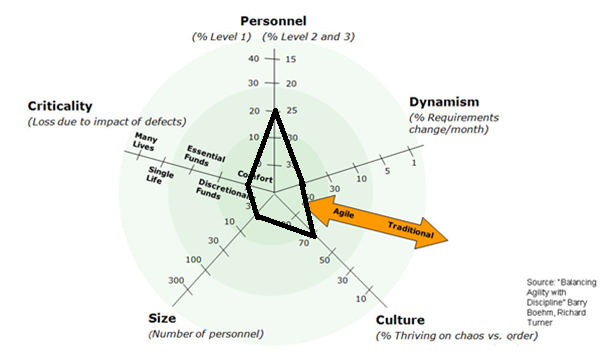
\includegraphics[scale=0.32]{includes/billeder/bohmsmodel.png}
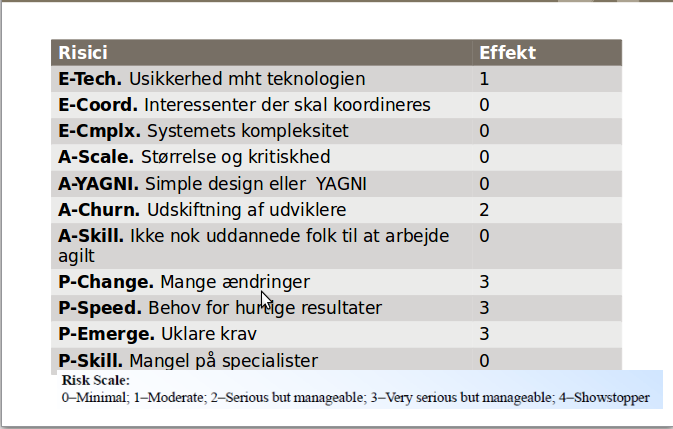
\includegraphics[scale=0.32]{includes/billeder/risici_analyse.png}

\begin{center}
\line(1,0){450}
\end{center}

\subsubsection*{Android phone}
Omgivelser (Environment), E-risici mht. projektets omgivelser.
\begin{itemize}
\item E-Tech. Usikkerhed mht. teknologien: 2 
\begin{itemize}
\item Android ide: 2
\item Versionstyring: 3
\item Emulator: 1
\end{itemize}

\item E-Coord. Interessenter der skal koordineres: 0
\item E-Cmplx. Systemets kompleksitet: 2
\begin{itemize}
\item FoodMap funktionalitet: 2
\item API: 1
\end{itemize}

\item A-Scale. St�rrelse og kritiskhed: 0
\item A-YAGNI. Simpelt design eller YAGNI: 1
\item A-Churn. Udskiftning af udviklere: 0
\item A-Skill. Ikke nok uddannelse af folk til at arbejde agilt: 3
\item P-Change. Mange �ndringer: 1
\item P-Speed. Behov for hurtige resultater: 2
\item P-Emerge. Uklare krav: 1
\item P-Skill. Mangel p� specialister: 3
\end{itemize}

\begin{center}
\line(1,0){450}
\end{center}

\begin{center}
\line(1,0){450}
\end{center}

\subsubsection*{Windows phone} 
\begin{itemize}
\item E-Tech. Usikkerhed mht teknologien: 1
\item E-Coord. Interessenter der skal koordineres: 1
\item E-Cmplx. Systemets kompleksitet: 0
\item A-Scale. St�rrelse og kritiskhed: 0
\item A-YAGNI. Simpelt design elller YAGNI: 4
\item A-Churn. Udskiftning af udviklere: 0
\item A-Skill. Ikke nok uddannelse af folk til at arbejde agilt: 3
\item P-Change. Mange �ndringer: 0
\item P-Speed. Behov for hurtige resultater: 1
\item P-Emerge. Uklare krav: 1
\item P-Skill. Mangel p� specialister: 3
\end{itemize}

\begin{center}
\line(1,0){450}
\end{center}

Database